\documentclass{article}
\usepackage{spconf,amsmath,graphicx}
\usepackage{amssymb}

\usepackage{tikz}
\usetikzlibrary{arrows,decorations.pathmorphing,backgrounds,fit,petri, decorations.pathreplacing,shadows,calc}
\usetikzlibrary{shapes.geometric}
\usetikzlibrary{shapes}
\usetikzlibrary{positioning}

\usepackage{fancyhdr}

\fancyhf{}
\fancyhead[C]{
\textcolor{red}{\scriptsize
© 2023 IEEE. Personal use of this material is permitted. Permission from IEEE must be obtained for all other uses, in any current or future media, including reprinting/republishing this material for advertising or promotional purposes, creating new collective works, for resale or redistribution to servers or lists, or reuse of any copyrighted component of this work in other works.}
}
\renewcommand\headrulewidth{0pt}
\pagestyle{fancy}
\headsep 1cm

\usepackage{array}
\newcolumntype{?}{!{\vrule width 2pt}}

\usepackage{hyperref}
\definecolor{urlcolor} {rgb}{0,0,0.9333333333333}
\hypersetup{
    colorlinks=true,     
    urlcolor=urlcolor,
    linkcolor=black,
    filecolor=black,
    citecolor=black,
    menucolor=black,
    runcolor=black
    }

\usepackage{xcolor,soul,framed}
\newcommand{\luc}[1]{\mbox{ }\newline\begin{minipage}{.8\columnwidth}\color{red}\small \textbf{Luc: } #1\end{minipage}}
\newcommand{\alexis}[1]{\mbox{ }\newline\begin{minipage}{.8\columnwidth}\color{cyan}\small \textbf{Alexis : }#1\end{minipage}}
\newcommand{\olivier}[1]{\mbox{ }\newline\begin{minipage}{.8\columnwidth}\color{violet}\small \textbf{Olivier : }#1\end{minipage}}
\newcommand{\mathieu}[1]{\mbox{ }\newline\begin{minipage}{.8\columnwidth}\color{olive}\small \textbf{Mathieu : }#1\end{minipage}}
\newcommand{\florian}[1]{\mbox{ }\newline\begin{minipage}{.8\columnwidth}\color{orange}\small \textbf{Florian : }#1\end{minipage}}

\makeatletter
\newcommand\footnoteref[1]{\protected@xdef\@thefnmark{\ref{#1}}\@footnotemark}
\makeatother

\hyphenation{Log-Euclidean}

\title{Structure-Preserving Transformers for Sequences of SPD Matrices}
\name{Mathieu Seraphim \qquad
Alexis Lechervy \qquad
Florian Yger  \qquad
Luc Brun \qquad
Olivier Etard
\thanks{The first author is supported by the French National Research Agency (ANR) and Region Normandie under grant HAISCoDe. This work was granted access to the HPC resources of IDRIS under the allocation 2022-AD010613618 made by GENCI, and to the computing resources of CRIANN (Normandy, France).}}
\address{ Normandie Univ, UNICAEN, ENSICAEN, CNRS, GREYC, 14000 Caen, France \\
       LAMSADE, CNRS, PSL Université Paris-Dauphine, France \\
      \hspace{-7px} Normandie Université, UNICAEN, INSERM, COMETE, CYCERON, CHU Caen, 14000, Caen, France}


\begin{document}

\maketitle

\begin{abstract}
In recent years, Transformer-based auto-attention mechanisms have been successfully applied to the analysis of a variety of context-reliant data types, from texts to images and beyond, including data from non-Euclidean geometries. In this paper, we present such a mechanism, designed to classify sequences of Symmetric Positive Definite matrices while preserving their Riemannian geometry throughout the analysis. We apply our method to automatic sleep staging on timeseries of EEG-derived covariance matrices from a standard dataset, obtaining high levels of stage-wise performance.
\end{abstract}

\begin{keywords}
Transformers, SPD Matrices, Structure-Preserving, Electroencephalography, Sleep Staging
\end{keywords}

\section{Introduction}
\label{sec:intro}

When analyzing the relationship between feature vectors or concurrent signals, correlation and covariance matrices are a useful tool. Such matrices are at least Positive Semi-Definite, and often fully Symmetric Positive Definite (SPD).
The set of  SPD matrices () is a non-Euclidean, Riemannian (i.e. metric) manifold, and the regular Euclidean operations of most Neural Network (NN)-based models seldom preserve that geometric structure, introducing deformations such as the ``swelling effect"~\cite{LogEuclidean}.
Structure-preserving NN-based approaches have been introduced~\cite{huang2017spdnet,manifoldnet}, deriving their layers from one of two geodesic-defining metrics on . Affine invariant metrics offer the best properties, but present computational challenges (e.g. no closed-form formula for averaging)~\cite{affine_invariant}. 
LogEuclidean metrics are less isotropic, but still prevent swelling while being easier to compute~\cite{LogEuclidean}. With , we chose this LogEuclidean distance:

This metric relies on the matrix logarithm , bijectively and isometrically mapping  onto , the vector space of  symmetric matrices (with  being its inverse).
Here,  is the  norm applied to the upper triangular of .
LogEuclidean operations are thus the Riemannian equivalent to Euclidean operations on .

\begin{figure}
  \begin{center}
  \resizebox{0.4\textwidth}{!}{
		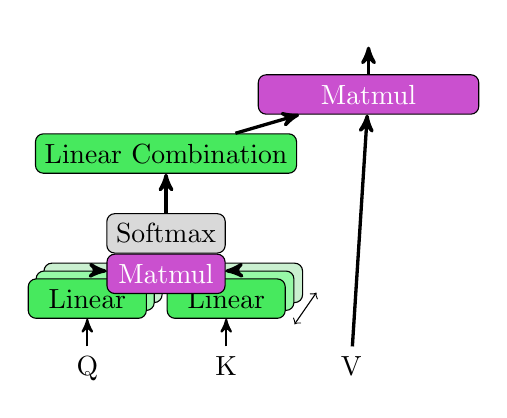
\begin{tikzpicture}
			\definecolor{colorMatMul}{RGB}{202,80,207}
			\colorlet{colorSoftMax}{black!15}
                \definecolor{LinearFront}{RGB}{71,233,94}
                \definecolor{LinearMid}{RGB}{151,249,167}
                \definecolor{LinearBack}{RGB}{202,240,208}
                \definecolor{LinearCombi}{RGB}{71,233,94}
                
   
			\node[align=center] (Q){Q};
			
			\node[minimum width = 1.5cm, minimum height = 0.5cm,align=center, rectangle, draw=black,xshift=0.2cm,fill=LinearBack,opacity=1,above = 0.55cm of Q,rounded corners=0.1cm] (L1_3){};
			\node[minimum width = 1.5cm, minimum height = 0.5cm,align=center, rectangle, draw=black,xshift=0.1cm,fill=LinearMid,opacity=1,above = 0.45cm of Q,rounded corners=0.1cm] (L1_2){};						
			\node[minimum width = 1.5cm, minimum height = 0.5cm,align=center, rectangle, draw,fill=LinearFront,opacity=1,above = 0.35cm of Q,rounded corners=0.1cm] (L1){Linear};

			
			\node[minimum width = 1.5cm, minimum height = 0.5cm,align=center, rectangle, draw=black,xshift=0.2cm,fill=LinearBack,opacity=1,yshift=0.2cm, right = 0.27 cm of L1,rounded corners=0.1cm] (L2_3){};
			\node[minimum width = 1.5cm, minimum height = 0.5cm,align=center, rectangle, draw=black,xshift=0.1cm,fill=LinearMid,opacity=1,yshift=0.1cm, right = 0.26 cm of L1,rounded corners=0.1cm] (L2_2){};
			\node[minimum width = 1.5cm, minimum height = 0.5cm,align=center, rectangle, draw=black,fill=LinearFront,opacity=1, right = 0.25 cm of L1,rounded corners=0.1cm] (L2){Linear};

			\node[below = 0.35cm of L2,align=center] (K){K};
			
			\node[minimum width = 1.5cm, minimum height = 0.5cm,align=center, rectangle, draw=black, yshift=1.2 cm,rounded corners=0.1cm,fill=colorMatMul,text=white] (M1) at (,0){Matmul};
			
			\node[minimum width = 1.5cm, minimum height = 0.5cm,align=center, rectangle, draw=black, above = 0 cm of M1,rounded corners=0.1cm,fill=colorSoftMax] (Softmax){Softmax};			

			\node[minimum width = 3cm, minimum height = 0.5cm,align=center, rectangle, draw,fill=LinearCombi, above = 0.5 cm of Softmax,rounded corners=0.1cm] (L3){Linear Combination};			
			\node[minimum width = 2.8cm, minimum height = 0.5cm,align=center, rectangle, draw=black, right = -0.5 cm of L3, yshift = 0.75 cm,rounded corners=0.1cm,fill=colorMatMul,text=white] (M2){Matmul};			
			
\node[align=center,right = 1.07cm of K] (V){V};
			\node[align=center,above = 0.35cm of M2] (Vide){};
\draw[->, thick, >=stealth'](Q.north) -- (L1.south)node[right,midway]{\fontsize{3}{6}\selectfont };;
			\draw[->, thick, >=stealth'](K.north) -- (L2.south);


			\draw[->, very thick, >=stealth'](V) -- (M2)node[right,midway]{\fontsize{3}{6}\selectfont };
		
			\draw[->, very thick, >=stealth'](L3) -- (M2)node[left,midway]{\fontsize{3}{6}\selectfont };
			
			\node[right = -0.1cm of L2,yshift=-0.45cm] (L2_d){};
			\node[right = 0.13cm of L2_3] (L2_3d){};
			\draw[<->,yshift=10cm](L2_d) -- (L2_3d)node[right,midway]{\fontsize{3}{6}\selectfont };
			
			\draw[->, very thick, >=stealth'](L1_2.north) -- (M1);
			\draw[->, very thick, >=stealth'](L2_2.north)  -- (M1)node[right,midway]{\fontsize{3}{6}\selectfont 
				
				};
			
			\draw[->, very thick, >=stealth'](Softmax.north) -- (L3.south)node[right,midway]{\fontsize{3}{6}\selectfont };
			
			\draw[->, very thick, >=stealth'](M2.north) -- (Vide.south)node[right,midway]{\fontsize{3}{6}\selectfont };
\end{tikzpicture}
	}      \caption{The SP-MHA architecture. In parentheses are tensor dimensions at every step, with  the batch size.}
  \label{fig:SPMHA}
  \end{center}
\end{figure}

\begin{figure*}
  \begin{center}
  \includegraphics[width=.9\textwidth]{model_architecture.pdf}
  \caption{SPDTransNet global architecture, with  feature tokens per epoch.}
  \label{fig:architecture}
  \end{center}
\end{figure*}

In this paper, we present a structure-preserving self-attention mechanism applicable to sequences of SPD matrices, derived from the aforementioned LogEuclidean metric. We embed said mechanism into a Transformer-based architecture, and apply it to a biomedical classification problem.
Transformer-based technology has exploded in popularity ever since its introduction in~\cite{transformers}, with self-attention mechanisms being applied to very different problems.
With regards to Riemannian geometry, innovations seem centered around the computation and application of attention maps, specifically. For instance, Konstantinidis et al.~\cite{Konstantinidis2022MultimanifoldAF} combine the standard attention maps with Grassmann and SPD manifold-valued maps, to enrich their computer vision model's descriptive capabilities. By contrast, both He et al.~\cite{he_gauge_equivariant} and Li et al.~\cite{li2022geodesic} developed architectures to analyze 2D-manifold-valued data in 3D space, the former achieving rotational equivariance with respect to surfaces on the manifold and the latter developing two geodesic distances applicable to point clouds, and building attention maps from these distances. More generally, Kratsios et al.~\cite{kratsios2022universal} provide a mathematical framework to apply attention mechanisms on a variety of constrained sets, including manifolds.
While the latter approaches share our interest in preserving geometric information, little to no focus is given to a Transformer's other components. As far as we are aware, ours is the only approach to apply structure-preserving Transformers to SPD manifold-valued data.


\section{SPD Structure-Preserving Attention}
\label{sec:theory}

Let  be the the canonical basis of , with , and all other coefficients at 0. Let the triangular number  be the dimension of .
Any matrix  of  can be written in the basis  as a vector (a.k.a. ``token") of coordinates in . Therefore, any linear combination of these tokens would equate to the same linear combination in , and thus to a LogEuclidean weighted sum in , preserving its manifold structure.


\subsection{Structure-Preserving Multihead Attention (SP-MHA)}
\label{ssec:SPMHA}

In the original Linear Multihead Attention (L-MHA) component of Transformers~\cite{transformers}, the input tokens in the Q, K and V tensors are processed in parallel in  attention heads, then recombined through concatenation.
There is no guarantee that any underlying SPD structure in our tokens would survive this concatenation. Echoing the similar concerns, Li et al.~\cite{li2022geodesic} decided to forego having multiple heads. We chose instead to redefine the bloc, keeping the parallel attention maps computation without sacrificing our data's structure.

Let  be the dimension of input tokens.
As seen in Figure~\ref{fig:SPMHA}, our SP-MHA bloc does the following:

with  and  banks of  linear maps from  to ,  the softmax function, and  the weighted linear combination of the  post-softmax attention maps.
Although said attention maps are identical to their L-MHA counterparts, the only operation applied to V is the final matrix multiplication, i.e. linear combinations of V's tokens weighted by the combined attention map, which do not threaten our tokens' vector space geometry.

\subsection{Triangular linear maps}
\label{ssec:justification}

Let  and  have the canonical bases  and , respectively. Let  be a linear map from  to , represented by the matrix  in  with respect to the bases (implemented in code through a fully connected NN layer between tokenized matrices). We shall refer to such a map as a ``triangular" linear map.

Let  be in , mapped to  through . As  is a continuous linear map:


with  the matrix norm induced by the norm , and  mapping  onto .
By definition of  (Equation~\ref{eq:LE}), Equations~\ref{eq:ineq_1} and~\ref{eq:ineq_2} are strictly identical.
Hence, applying  on our tokens is equivalent to applying  on matrices in . The output tokens exhibit the Riemannian structure of , and relations of proximity are preserved. Therefore, so is the overall structure of our data.

Note that while other SPD-to-SPD NN-based mappings have been proposed~\cite{SPD_dim_reduc,huang2017spdnet}, they rely on full-rank weight tensors, whereas  does not require special constraints.

\begin{table*}[ht]
\small
\centering
\begin{tabular}{ |c|c?c|c|c?c|c|c| }
    \cline{2-8}
    \multicolumn{1}{c|}{} & Model & MF1 & Macro Acc. & N1 F1 & Valid. metric & Token dim.  & \# Feat. Tokens  \\\hline
    1 & DeepSleepNet~\cite{Supratak2017} & 78.14  4.12 & 80.05  3.47 & 53.52  8.24 & N/A & N/A & N/A \\\hline
    2 & IITNet~\cite{SEO2020102037} & 78.48  3.15 & 81.88  2.89 & 56.01  6.54 & N/A & N/A & N/A \\\hline
    3 & GraphSleepNet~\cite{jia2020graphsleepnet} & 75.58  3.75 & 79.75  3.41 & 50.80  8.06 & N/A & N/A & N/A \\\hline
    4 & Dequidt et al.~\cite{paul} & 81.04  3.26 & 82.59  3.45 & 58.42  6.09 & N/A & N/A & N/A \\\hline
    5 & Seraphim et al.~\cite{CAIP_article} & 79.78  4.56 & 81.76  4.61 & 58.43  6.41 & MF1 & Concatenation & 1 \\\hline
    6 & SPDTransNet,  & 81.06  3.49 & \textbf{84.87}  2.47 & 60.39  6.77 & MF1 & 351 () & 7 \\\hline
    7 & SPDTransNet,  & \textbf{81.24}  3.29 & 84.40  2.61 & \textbf{60.50}  6.18 & MF1 & 351 () & 10 \\\hline
    8 & SPDTransNet,  & 80.83  3.40 & 84.29  2.65 & 60.35  6.01 & N1 F1 &  351 () & 5 \\\hline
\end{tabular}
\caption{Results obtained from both our model and the re-trained literature. Best results are in \textbf{bold}.}
\label{tab:results}
\end{table*}

\section{Application to EEG Sleep Staging}
\label{sec:EEG}

The study of sleep most often requires the analysis of electrophysiological - including electroencephalographic (EEG) - signals, subdivided into fixed-length windows (``epochs") and manually labeled with the appropriate sleep stages, inferred from properties of the signal in and around each epoch~\cite{berry2017aasm}.

As seen in a recent survey by Phan et al.~\cite{Phan_survey}, state-of-the-art automatic sleep staging models typically use two-step architectures -  given a sequence of epochs, epoch-wise features are extracted before being compared at the sequence-wise level, utilizing this contextual information to improve classification.
Since epochs often contain markers indicative of multiple stages, two-step architectures tend to subdivide them further, extracting features from subwindows using convolutional NNs~\cite{SEO2020102037} and/or recurrent NNs~\cite{phan2022xsleepnet,phan2023lseqsleepnet} - the latter utilizing RNNs for both steps.
Multiple authors have adapted this context-inclusive approach to Transformer-based architectures~\cite{zhu2020,phan2022sleeptransformer,CAIP_article}, with auto-attention mechanisms at both the intra- and inter-epoch levels, taking advantage of the high performance they offer when applied to sequence-based data.

\subsection{Improving stage-wise classification}
\label{ssec:N1_performance}

According to the aforementioned survey~\cite{Phan_survey}, current sleep staging models have attained a sufficient performance level to replace manual staging in some contexts. However, we have found that class-wise performance was often lacking, particularly with regards to the N1 sleep stage~\cite{berry2017aasm}, universally difficult to classify (Section~\ref{sec:experiments}).
Most EEG datasets are heavily imbalanced, with the N1 stage often underrepresented (Section~\ref{ssec:dataset}) - models optimized for high overall accuracy may thus sacrifice N1 classification if it improves global performance.
To account for this, recent approaches~\cite{paul,CAIP_article} elected to primarily evaluate their performance through the macro-averaged F1 (MF1) score, a class-wise balanced metric widely used in the literature. They also rebalance their training sets through oversampling, so that all stages within have the same number of classification targets.
While the survey states that a sequence-to-sequence classification scheme (classifying each epoch in the input sequence) might lead to better performance, having multilabel inputs is nonsensical for this rebalancing - hence their use of a sequence-to-epoch scheme (classifying one epoch per sequence).

Seraphim et al.~\cite{CAIP_article} hypothesized that an analysis through functional connectivity - the activation correlations between different brain regions~\cite{EICKHOFF2015187} - enhances stage-wise performance. Such an analysis was first done by Jia et al.~\cite{jia2020graphsleepnet}, using epoch-wise graph learning to estimate said connectivity and sequence-wise spatio-temporal graph NNs to compare them.
By contrast, Seraphim et al. estimate it through covariance matrices.
Their two-step model uses standard Transformer encoders at each step, reminiscent of~\cite{phan2022sleeptransformer}. Each input epoch is described as a multichannel timeseries of SPD matrices, which are then tokenized bijectively.
However, their approach does not guarantee the preservation of their data's SPD structure, as they operate a channel-wise concatenation of their tokens, in addition to the concatenations found within their encoders (Section~\ref{ssec:SPMHA}).
Hence, we propose a Transformer-based model capable of analyzing EEG-derived functional connectivity through SPD matrices \textit{without} sacrificing the SPD structure of our data throughout the analysis.

\subsection{The SPDTransNet model}
\label{ssec:model}

As can be seen in Figure~\ref{fig:architecture}, our SPDTransNet model takes as input a sequence of  epochs, composed of a central epoch to classify and surrounding epochs to provide context.
Given  the context size, we have .

Each EEG signal is decomposed into  channels, divided into epochs, and further subdivided into  subwindows per epoch. After preprocessing (Section~\ref{ssec:dataset}), each epoch is described by  matrices in .
Each matrix is mapped onto  logarithmically (Section~\ref{sec:intro}), tokenized (Section~\ref{sec:theory}), and linearly mapped onto  (with , as we have found that larger tokens improve performance).
The  grid of tokens is then arranged into a 1D sequence, with the  tokens in the channel 1 followed by the  tokens in channel 2, etc.

At the intra-epoch level, a first positional encoding is applied to the tokens, which pass through the first Transformer encoder. The  output tokens are then uniformly divided into  groups, with each group averaged into a single token.
The  sets of  tokens are then regrouped at the inter-epoch level, and passed through another positional encoding and Transformer encoder pair.
Finally, the  tokens corresponding to the central epoch (of index  in Figure~\ref{fig:architecture}) go through two FC blocs\footnote{Fully connected layers followed by ReLU activation and dropout layer.}, and are mapped onto  by a final classification linear map, with  the number of classes.

We ensure structure preservation by using the SP-MHA bloc in all Transformer encoders, and choosing all linear maps within said encoders' Feed-Forward (FF) components~\cite{transformers} and the aforementioned FC blocs to be triangular (Section~\ref{ssec:justification}).
The ReLU and dropout layers in the FF and FC blocs do not cause issue, as setting a values within a token to 0 won't remove the corresponding matrix from .
Same for the positional encodings, average poolings and in-encoder layer normalizations, which all qualify as linear combinations.

As such, our model preserves the SPD structure of its input up to the final classification map.

\subsection{Dataset and preprocessing}
\label{ssec:dataset}

We utilize the MASS SS3 dataset~\cite{o2014montreal} due to its large number of available EEG electrode-derived signals and widespread use in the literature. It is composed of 62 full-night recordings of healthy subjects, segmented into 30s epochs. Due to its nature, it is unbalanced, with the largest and smallest of its  classes (stages N2 and N1) composed of 50.24\% and 8.16\% of the dataset, respectively.
As do~\cite{paul} and~\cite{CAIP_article}, we selected the 8 electrodes F3, F4, C3, C4, T3, T4, O1 and O2.

To estimate functional connectivity from those signals, we apply the same preprocessing pipeline as~\cite{CAIP_article}\footnote{\label{fn:Git}More details at github.com/MathieuSeraphim/SPDTransNet.}, computing  covariance matrices in , with  the sequence length and  the number of frequency-based channels. We then augment our matrices with signal-derived information before whitening them\footnoteref{fn:Git}, leading to more uniformly distributed matrices in  (i.e. ).
Said whitening requires the computation of average covariance matrices per recording and channel, which was done in~\cite{CAIP_article} by computing the covariances over the entire recording. Instead, we average all relevant matrices using the standard affine invariant metric~\cite{affine_invariant}, improving performance.

\section{Experiments \& Results}
\label{sec:experiments}

To maximize class-wise performance, we operate a hyperparameter research per configuration, followed by a 31-fold cros-validation. As do~\cite{paul,CAIP_article} (Section~\ref{ssec:N1_performance}), we rebalance all training sets and maximize the MF1 score. 
To explore the importance of the context length  (Section~\ref{ssec:model}) within our model, we ran hyperparameter researches with  = 6, 10 or 14 (i.e.  = 13, 21 or 29), with hyperparameter research configuration unchanged between them.

Our hyperparameter researches use the Optuna tool~\cite{akiba2019optuna}, with 5 simultaneous runs and 50 total runs per configuration. Hyperparameters include\footnoteref{fn:Git} the token size , set by the first linear map (Section~\ref{ssec:model}) and chosen in \{351, 378\} (i.e.   \{26, 27\})\footnote{\label{fn:d/h}Since  must be an integer, potential values for those are limited.};
the  parameter of each Transformer encoder, in \{3, 9\}\footnoteref{fn:d/h};
and the number of epoch feature tokens  (Section~\ref{ssec:model}), chosen among \{1, 3, 5, 7, 10\} - with in particular  akin to describing each epoch with a single token, and  corresponding to one token being preserved per channel.
We train all folds on the hyperparameters giving the best validation MF1, as well as those with the best F1 score for the N1 stage. Out of those two sets, the results from the set yielding the best average test MF1 is presented in lines 6 to 8 of Table~\ref{tab:results}, with the corresponding hyperparameter set,  and  in the final three columns.

We compare ourselves to five models:
DeepSleepNet~\cite{Supratak2017}, often used as a benchmark, with a pre-trained epoch-wise global feature map submodel followed by a sequence-to-sequence RNN;
IITNet~\cite{SEO2020102037}, the source of our 31 folds, extracting multiple features per epoch through CNNs and comparing them through sequence-wise RNNs;
GraphSleepNet~\cite{jia2020graphsleepnet}, expliciting epoch-wise functional connectivity through graph learning;
Dequidt et al.~\cite{paul}, utilizing a single-step pretrained visual CNN, who both maximize MF1 performance and rebalance training sets;
and Seraphim et al.~\cite{CAIP_article}, with a similar approach to ours lacking in structural preservation (Section~\ref{ssec:N1_performance}).
These models were re-trained using our methodology - except for oversampling in DeepSleepNet's sequence-to-sequence submodel - though we use only their published hyperparameters.
Finally, as test sets vary between models due to sequence-based recording-wise border effects, we trim test set borders to enforce uniformity.
All these changes cause the results we obtained to differ somewhat from those initially published.
Our results, averaged over all folds, are displayed in lines 1 to 5 of Table~\ref{tab:results}.

As shown in Table~\ref{tab:results}, we obtain the best MF1 and N1 F1 scores for , whereas the best macro-averaged accuracy is obtained for .
For all values of , we outperform the state-of-the-art on the considered metrics (except for the MF1 score for ). Moreover, all three configurations have around a two-point lead in both macro accuracy and N1 F1 score.
While our model favors the smaller token size of  for all values of , it seems that having a large number of tokens to describe each epoch (at least ) is necessary for best performance. 
Overall,  seems to be a good compromise to capture enough contextual information without burdening our model with irrelevant data.

\section{Conclusion}
\label{sec:conclusion}

We presented SP-MHA, a novel, structure-preserving Multihead Attention bloc, and integrated it into our SPDTransNet model, designed to analyze SPD matrix sequences. We proved said model's capabilities through automatic EEG sleep staging, obtaining a high level of per-stage performance relative to the literature.
Beyond this two-step analysis, SPDTransNet can be easily adapted to a variety of problems, for instance by using only a single encoder step and/or implementing a sequence-to-sequence classification scheme.

\newpage
\bibliographystyle{IEEEbib_shortened_names}
\bibliography{biblio}

\end{document}
